\documentclass[11pt,compress,t,notes=noshow, xcolor=table]{beamer}


\input{../../style/preamble}
\input{../../latex-math/basic-math}
\input{../../latex-math/basic-ml}

\setbeamersize{text margin left=0.3cm,text margin right=0.3cm}


\title{Applied Machine Learning}
% \author{LMU}
%\institute{\href{https://compstat-lmu.github.io/lecture_iml/}{compstat-lmu.github.io/lecture\_iml}}
\date{}

\begin{document}

\titlemeta{
Time Series:
}{
Feature Engineering
}{
figure/bike_hourly_by_daytype
}{
\item Calendar and cyclic features
\item Lagged and rolling features
\item Feature importance and selection
}

% =========================================================
\section{Feature Engineering}
% ---------------------------------------------------------
\begin{vbframe}{Calendar Features}
  \vfill
  \begin{itemize}
    \item Day-of-Week, Day-of-Month, Week Number, Month, Quarter
    \item Boolean flags: public holidays, weekend, promotion days, end-of-month
  \end{itemize}
  \vspace{0.4cm}
  \begin{center}
    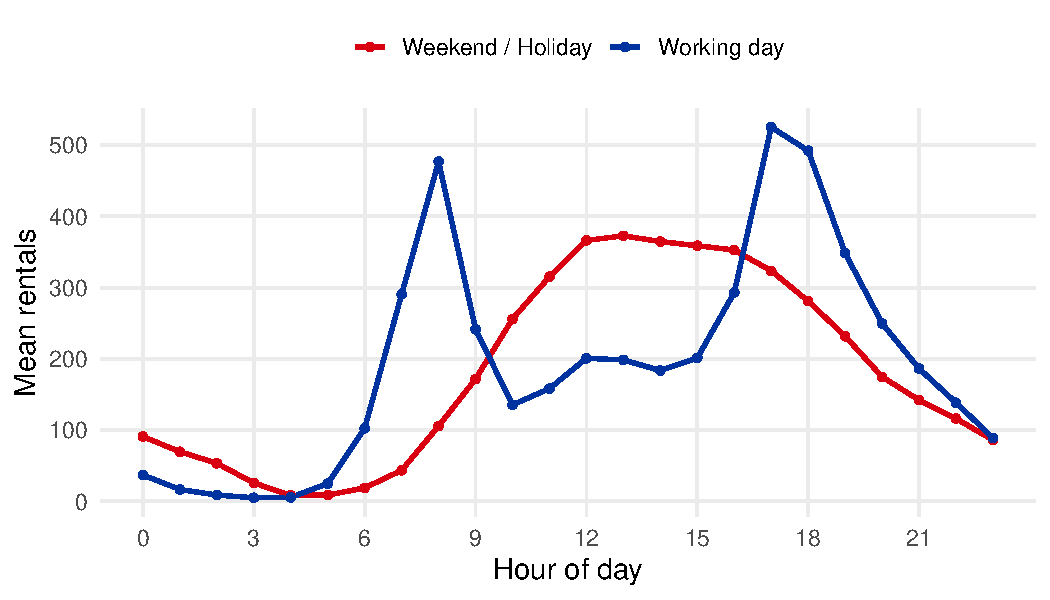
\includegraphics[width=0.55\textwidth]{figure/bike_hourly_by_daytype.pdf}
  \end{center}
  \vspace{-0.5em}
  \begin{block}{Why?}
    Capture human or process-driven periodicity. E.g., bike rentals peak on weekday mornings (commuters) but are spread throughout the day on weekends.
  \end{block}
  \vfill
\end{vbframe}

\begin{vbframe}{Cyclic Encoding}
  \vfill
  \[\text{sin}(2\pi \tfrac{hour}{24}),\; \text{cos}(2\pi \tfrac{hour}{24})\]
  \vfill
  \begin{itemize}
    \item Converts periodic integers (hour 0-23, month 1-12) into continuous space
    \item Eliminates artificial jump between 23 \(\rightarrow\) 0 (and December \(\rightarrow\) January)
    \item Most beneficial for linear and distance-based models; trees can often learn periodicity from raw integers but may need deeper splits to do so
  \end{itemize}
  \vfill
\end{vbframe}

\begin{vbframe}{Cyclic Encoding Visualization (Hour 0-23)}
  \begin{figure}
    \centering
    \begin{tikzpicture}[scale=2]
      % Axes
      \draw[->] (-1.2,0) -- (1.25,0) node[right] {$\cos(2\pi h/24)$};
      \draw[->] (0,-1.2) -- (0,1.25) node[above] {$\sin(2\pi h/24)$};
      % Unit circle
      \draw[gray!60] (0,0) circle (1);
      % Hour points
      \foreach \h in {0,...,23}{
        \coordinate (p) at ({cos(90-\h*15)},{sin(90-\h*15)});
        \fill[blue!70] (p) circle (1.3pt);
        \node[font=\tiny] at ($1.15*(p)$) {\h};
      }
    \end{tikzpicture}
  \end{figure}
\end{vbframe}

\begin{vbframe}{Lagged \& Auto-Regressive Features}
  \vfill
  \begin{itemize}
    \item Plain lags: $y_{t-1},\;y_{t-24},\;y_{t-168}$ (1 hour ago, yesterday, last week)
    \item Choose lag periods that match the data's seasonality (e.g., 168h = 1 week for hourly data)
    \item Multi-step: include future-known covariates (e.g., planned price, weather forecast)
    \item Combine with calendar features for interactions
  \end{itemize}
  \vfill
  \pause
\footnotesize
\begin{tabular}{llrrrrr}
\toprule
 & datetime & count & lag\_168 & lag\_336 & lag\_504 & lag\_672 \\
\midrule
17374 & 2012-12-31 19:00:00 & 119 & 18 & 507 & 564 & 692 \\
17375 & 2012-12-31 20:00:00 & 89 & 23 & 340 & 427 & 471 \\
17376 & 2012-12-31 21:00:00 & 90 & 22 & 200 & 300 & 300 \\
17377 & 2012-12-31 22:00:00 & 61 & 12 & 120 & 245 & 221 \\
17378 & 2012-12-31 23:00:00 & 49 & 11 & 54 & 126 & 144 \\
\bottomrule
\end{tabular}
\vfill
NB: The first $s$ rows have NaN for lag$\_s$. Options: drop those rows, impute, or use a model that handles NaN natively (\texttt{HistGradientBoostingRegressor} does).\\
Note: this table shows New Year's Eve -- lag\_168 is Christmas Eve, which explains the low values. Holidays create useful but noisy lag patterns.
\vfill
\end{vbframe}

\begin{vbframe}{Why Do Lags Work?}
\vfill
\begin{center}
  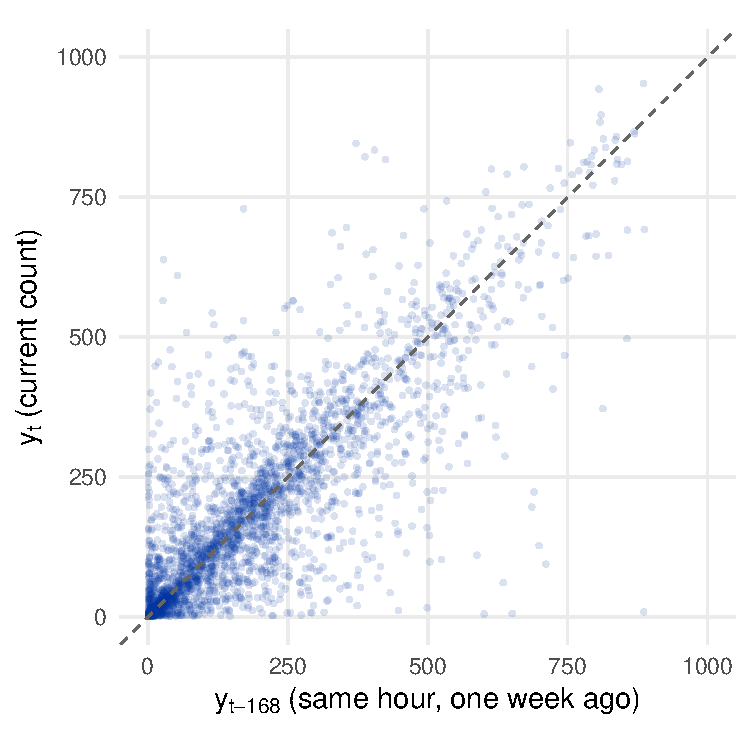
\includegraphics[width=0.55\textwidth]{figure/bike_lag168_scatter.pdf}
\end{center}
\vspace{-0.5em}
\footnotesize
$y_t$ vs $y_{t-168}$ (same hour, one week ago). The strong diagonal correlation shows that last week's count is a powerful predictor of this week's count.
\vfill
\end{vbframe}

\begin{vbframe}{Rolling / Expanding Statistics}
  \vfill
  Compute summary statistics over a sliding window of past observations:
  \begin{itemize}
    \item \textbf{Rolling mean / std}: $\bar{y}_{t,w} = \frac{1}{w}\sum_{i=t-w}^{t-1} y_i$ over window of size $w$
    \item \textbf{Rolling min / max}: capture recent extremes
    \item \textbf{Expanding mean}: $\bar{y}_{t} = \frac{1}{t-1}\sum_{i=1}^{t-1} y_i$ acts as a trend indicator
    \item \textbf{Percentiles}: 25th, 75th for distribution shape
  \end{itemize}
  \vfill
  Important: the window must only look \textbf{backward} (no future data!). When using lag features, shift the window by the forecasting horizon to avoid leakage.
  \vfill
\end{vbframe}

\begin{vbframe}{Interaction Features}
  \vfill
  Combine temporal features with covariates to capture conditional effects:
  \begin{itemize}
    \item Lag $\times$ Holiday flag $\rightarrow$ ``was the same hour last week also a holiday?''
    \item Weather $\times$ Weekend indicator $\rightarrow$ ``good weather on weekends drives leisure rentals''
    \item Hour $\times$ Workingday $\rightarrow$ commuter peaks only on working days
  \end{itemize}
  \vfill
  Tree-based models can learn interactions automatically, but explicit features can help simpler models and improve interpretability.
  \vfill
\end{vbframe}

\begin{vbframe}{Feature Importance \& Selection}
\vfill
With many engineered features, check which ones actually help:
\vfill
\begin{itemize}
    \item \textbf{Permutation importance}: shuffle one feature at a time, measure the drop in validation performance
    \item \textbf{Tree-based (impurity) importance}: built-in \texttt{feature\_importances\_} attribute (fast, but biased toward high-cardinality features; permutation importance does not have this bias)
    \item \textbf{SHAP values}: consistent, model-agnostic feature attributions (more expensive to compute)
\end{itemize}
\vfill
Rule of thumb: start with many features, inspect importance, prune correlated or weak ones.
\vfill
See the Interpretable Machine Learning course for more details on feature importance and model interpretation methods: \url{https://slds-lmu.github.io/iml/}
\vfill
\end{vbframe}

\begin{vbframe}{Putting It All Together: Raw Row $\rightarrow$ ML-Ready Row}
\vfill
\footnotesize
One row of the bike dataset \textbf{before} feature engineering:
\vspace{0.3em}

\begin{tabular}{lrrrl}
\toprule
holiday & temp & humidity & windspeed & datetime \\
\midrule
False & 24.6 & 0.45 & 0.30 & 2012-06-15 17:00 \\
\bottomrule
\end{tabular}

\vspace{0.8em}
The same row \textbf{after} feature engineering:
\vspace{0.3em}

\scriptsize
\begin{tabular}{lr|rr|rr|rr|r}
\toprule
holiday & temp & hour & dow\textsuperscript{*} & hour\_sin & hour\_cos & lag\_168 & lag\_336 & roll\_mean \\
\midrule
False & 24.6 & 17 & 4 & $-0.97$ & $-0.26$ & 432 & 389 & 285.3 \\
\bottomrule
\end{tabular}

\vspace{0.5em}
\normalsize
The datetime column is gone. All temporal information is now encoded as numeric features that any standard ML model can consume.\\
\textsuperscript{*}dow = day of week (Mon=0, Sun=6)
\vfill
\end{vbframe}


\endlecture
\end{document}
